\documentclass[11pt]{beamer}

%% Fonts
\usepackage{multicol}
\usepackage{mathabx}
\usepackage[scaled]{helvet}
\usepackage{lmodern}
\usepackage{eulervm}
\usefonttheme[onlymath]{serif}
\usefonttheme{professionalfonts}
\usefonttheme{structurebold}
\hypersetup{backref}
\usepackage{bm}
\usepackage{pgf}

%% Color & Theme
\definecolor{SUblue}{RGB}{0,0,180}
\usecolortheme[RGB={0,0,180}]{structure}
\usetheme{Boadilla}
\setbeamertemplate{navigation symbols}{}
\setbeamertemplate{itemize items}[circle]
\setbeamertemplate{enumerate items}[circle]
\setbeamerfont{title}{size=\large}
\setbeamerfont{frametitle}{size=\large}
\setbeamerfont{framesubtitle}{size=\large,shape =$\color{violet}{\looparrowdownright}~$}
\setbeamercolor{title}{fg=white, bg= SUblue!75!green}
\setbeamercolor{framesubtitle}{fg=violet}
\setlength{\leftmargini}{5pt}



\title[Research Days 2013]{Complex model to complex data}
\subtitle{--- the statistical approach}

\author[Feng Li]{\textbf{Feng Li}\\\texttt{ <feng.li@cufe.edu.cn>}}
\institute[StatMath, CUFE]{\footnotesize{\textbf{School of Statistics and
      Mathematics\\ Central University of Finance and Economics}}}
\date{}


%%%%%%%%%%%%%%%%%%%%%%%%%%%%%%%%%%%%%%%%%%%%%%%%%%%%%%%%%%%%%%%%%%%%%%%%%%%%%%%
\begin{document}


%% Title page
\begin{frame}[plain]
    \titlepage
  \tiny{Revision: \today}
\end{frame}



%% Outline page
% \section*{Outlines}
% \begin{frame}
%   \frametitle{Outlines}
%   \tableofcontents
% \end{frame}
%%%%%%%%%%%%%%%%%%%%%%%%%%%%%%%%%%%%%%%%%%%%%%%%%%%%%%%%%%%%%%%%%%%%%%%%%%%%%%%


\begin{frame}
\frametitle{Have you ever thought about...}

  \begin{itemize}
  \item Why the weather forecast is not accurate sometimes?\\
    (rain  or not $\Leftrightarrow$ cloudy, humidity, historical data)
  \item How does the email filter know whether a mail is a spam or not?\\
    (spam or not $\Leftrightarrow$ sender, keywords)
  \item Can we predict the next financial crisis?\\
    (Next crisis time $\Leftrightarrow$ when was last time, stock prices, exchange rate,
    unemployment rate)
  \item ...
  \end{itemize}
\vspace{1cm}
\emph{\textbf{Statistical modeling}} is trying to formalize (\textbf{model}) the relationships among the
variables (\textbf{data}).
\end{frame}

%\section{The trend of data we see}

\begin{frame}
\frametitle{Toy examples}
\framesubtitle{Father's height vs son's height}
      \begin{figure}
        \centering
        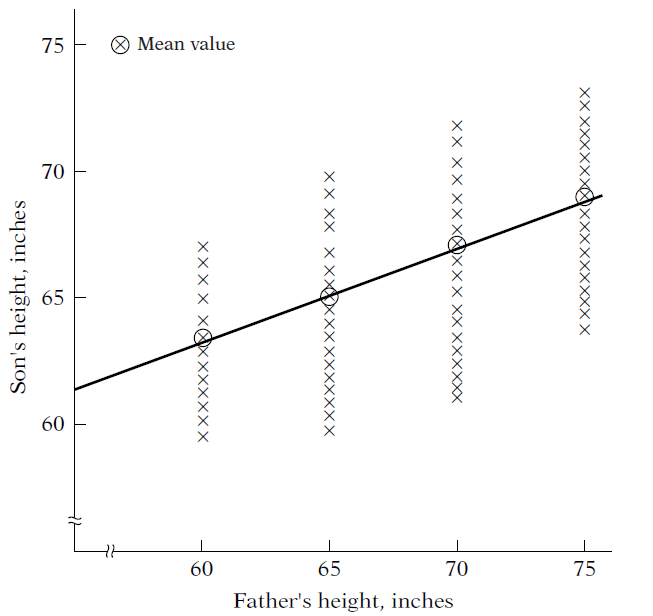
\includegraphics[height=0.7\textheight]{father_son.png}
      \end{figure}
\tiny{Gujarati, D. N. (2003). Basic Econometrics. 4th.}
\end{frame}

\begin{frame}
\frametitle{Toy examples}
\framesubtitle{Family income and consumption}
      \begin{figure}
        \centering
        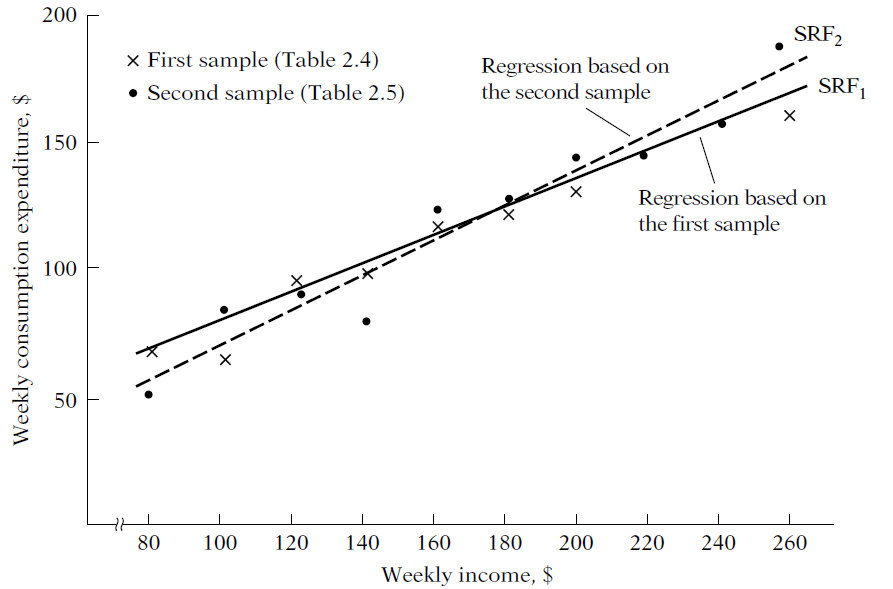
\includegraphics[height=0.7\textheight]{family_income_sample_line}
      \end{figure}
\tiny{Gujarati, D. N. (2003). Basic Econometrics. 4th.}
\end{frame}

\begin{frame}
  \frametitle{}
  \begin{itemize}
  \item Models are simple.
  \item Works well at most situations.
  \item Easy to imagine and implement.
  \item It takes less than 1 second to have the result with a laptop.
  \end{itemize}

\end{frame}

\begin{frame}
  \frametitle{The typical data in finance}
\framesubtitle{Daily stock market returns}
  \begin{figure}
    \centering
    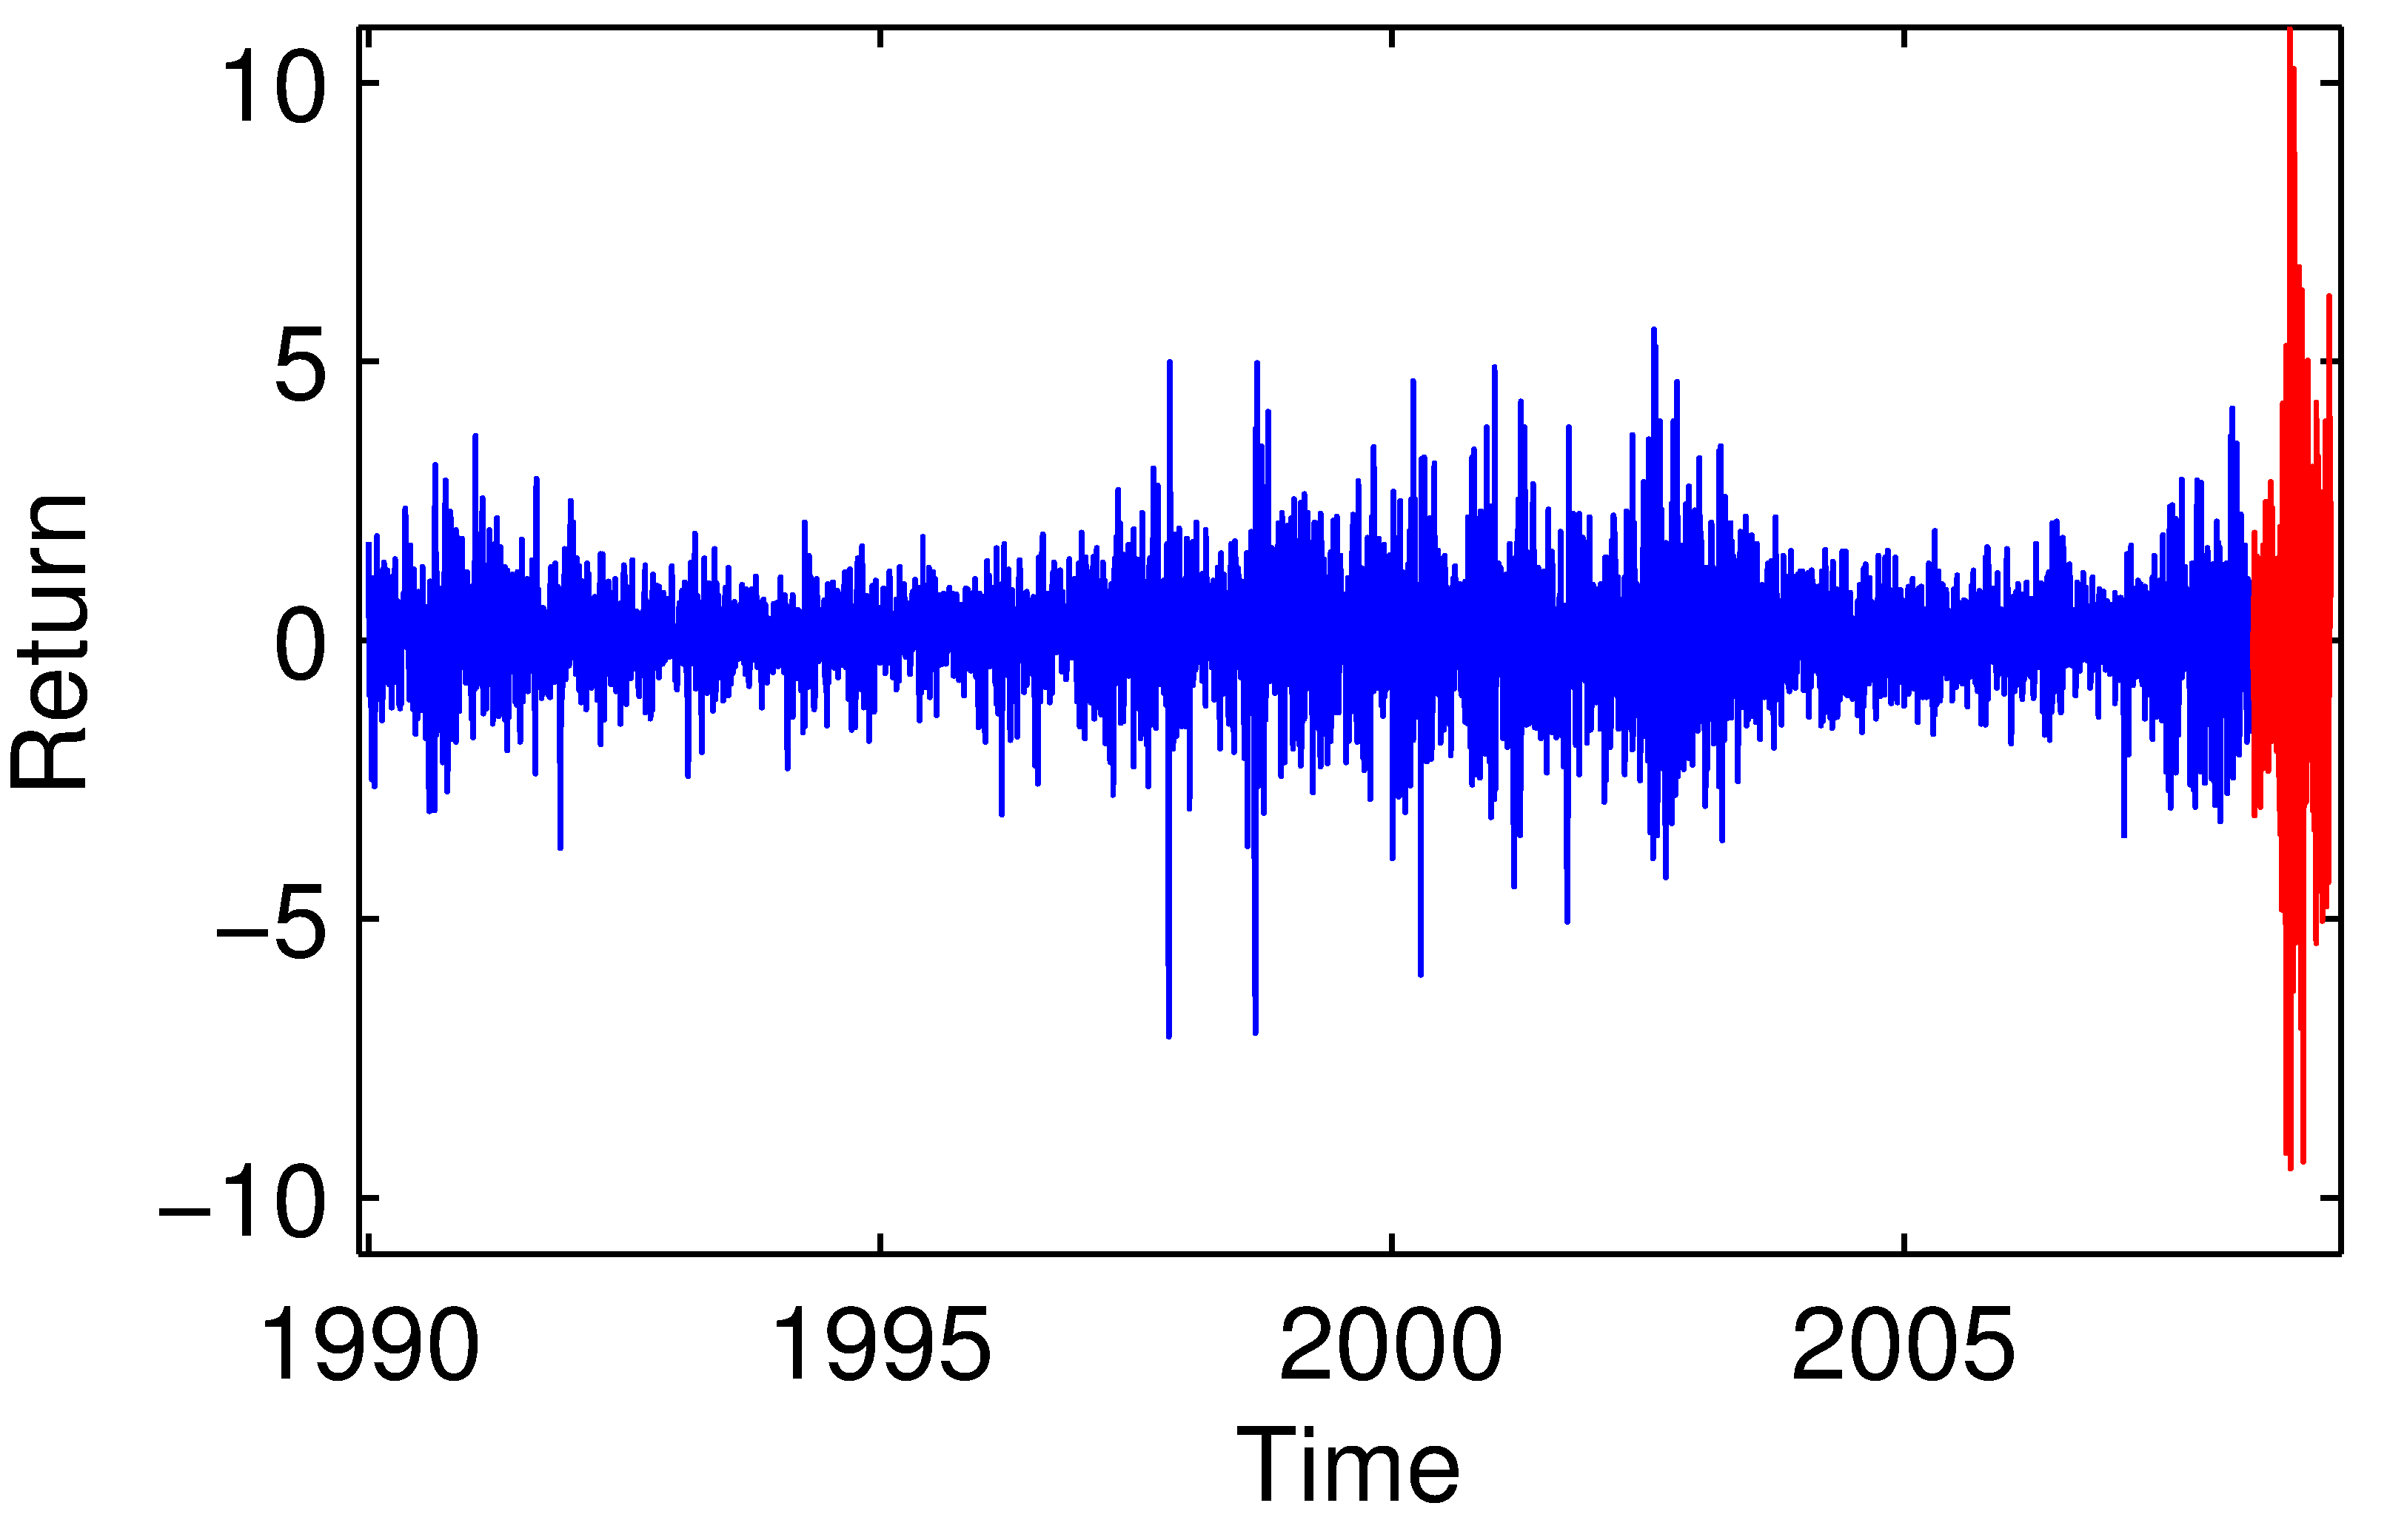
\includegraphics[height=0.8\textheight]{return}
  \end{figure}
\end{frame}


% \begin{frame}
%   \frametitle{The typical data in finance}
% \framesubtitle{Daily stock market returns}
%   \begin{figure}
%     \centering
%     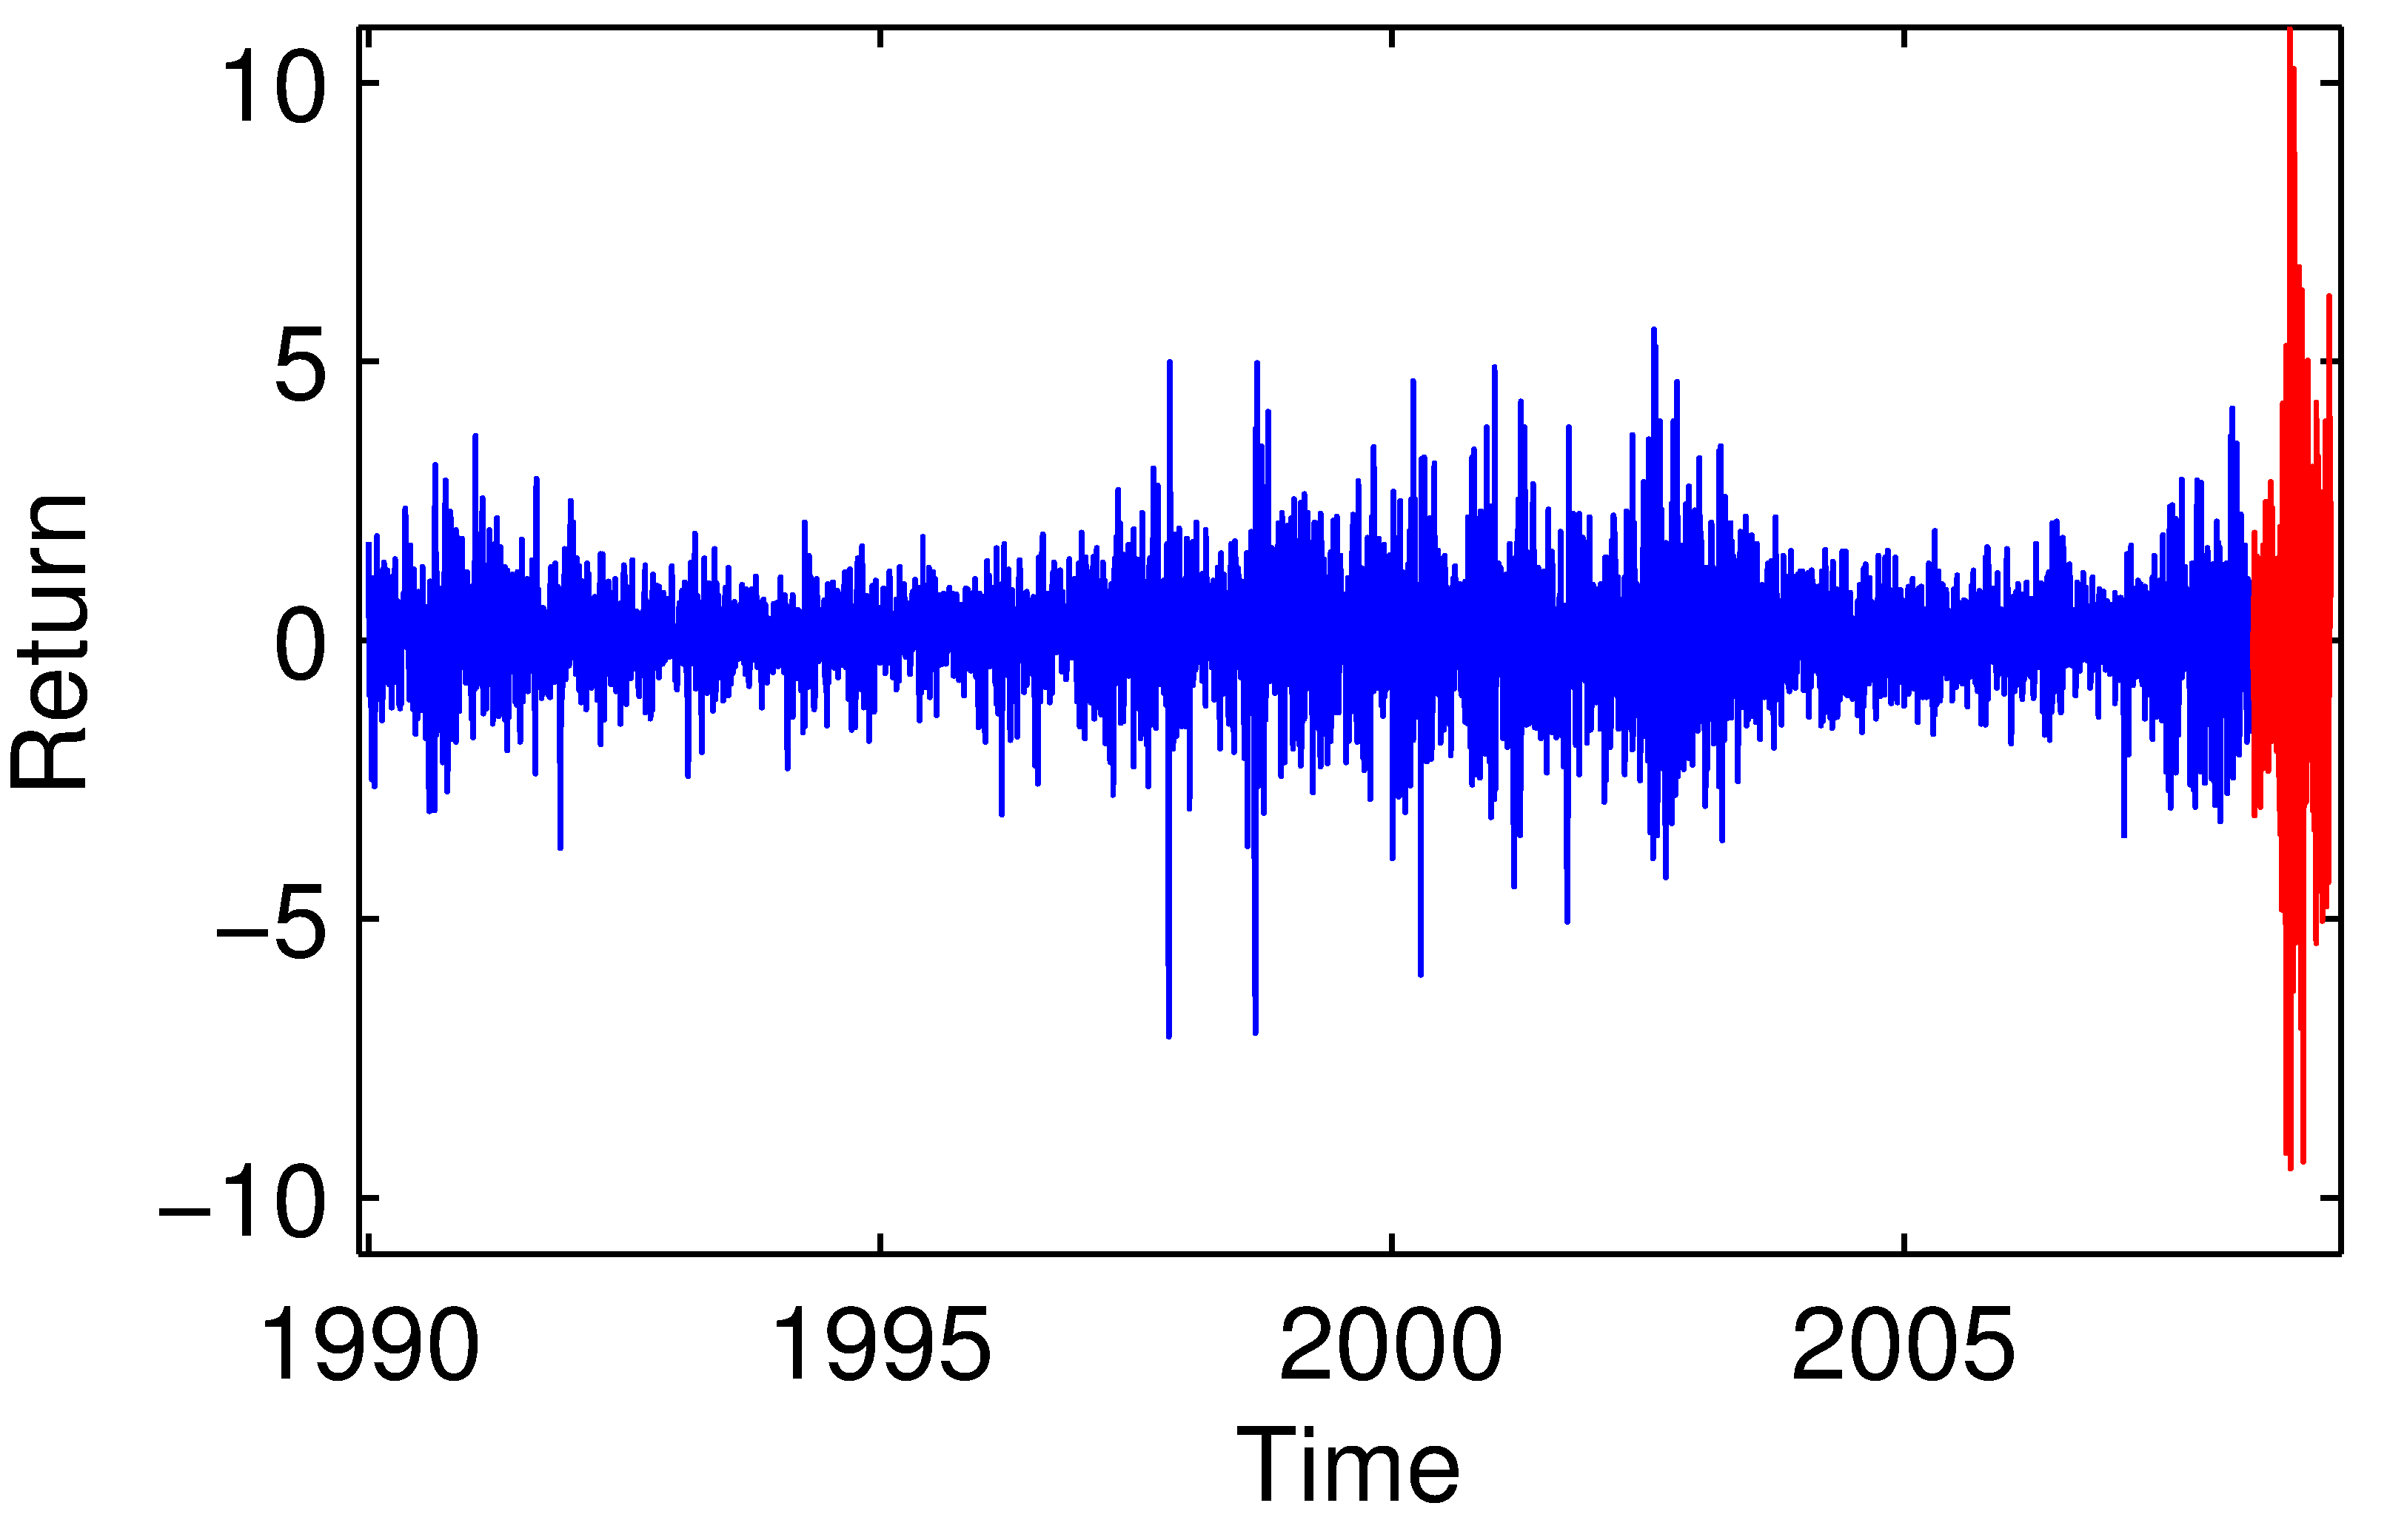
\includegraphics[height=0.8\textheight]{return}
%   \end{figure}
% \end{frame}


\begin{frame}
  \frametitle{The typical data in finance}
\framesubtitle{Daily stock market returns, a closer look}
  \begin{figure}
    \centering
    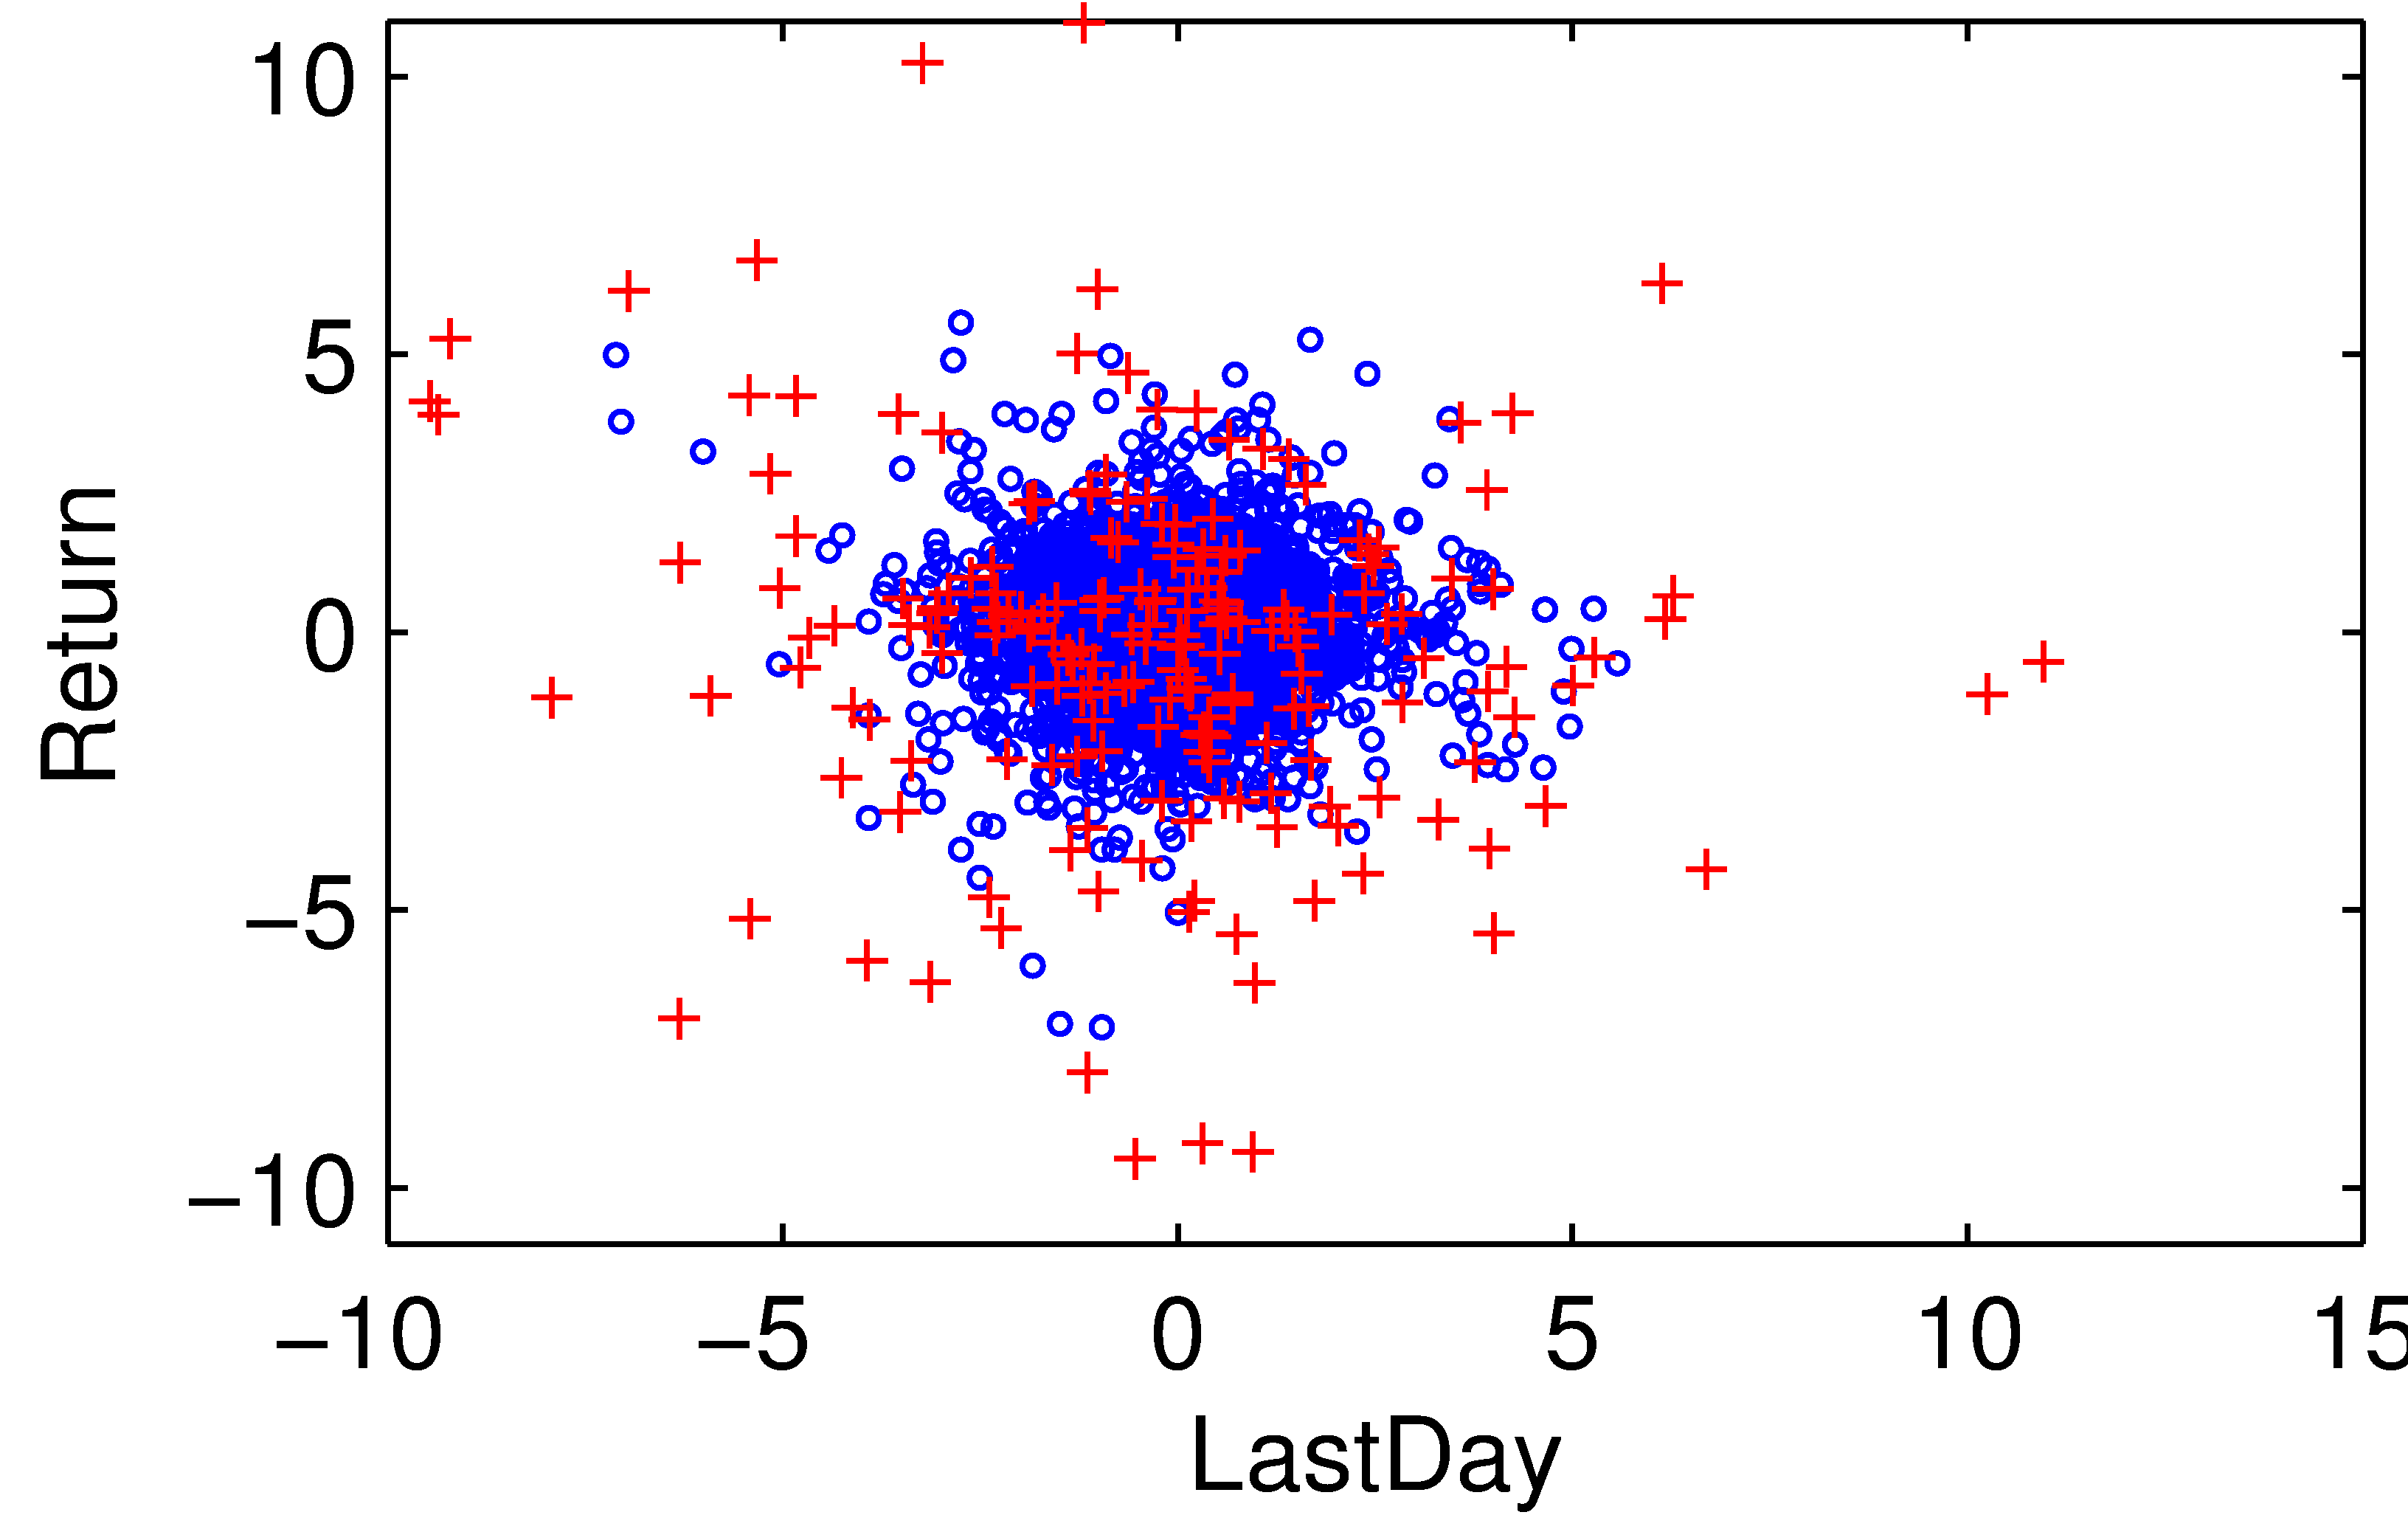
\includegraphics[height=0.8\textheight]{returnlastday}
  \end{figure}
\end{frame}

\begin{frame}
  \frametitle{The typical data in finance}
  \framesubtitle{Daily stock market returns, a closer look}
  \begin{figure}
    \centering
    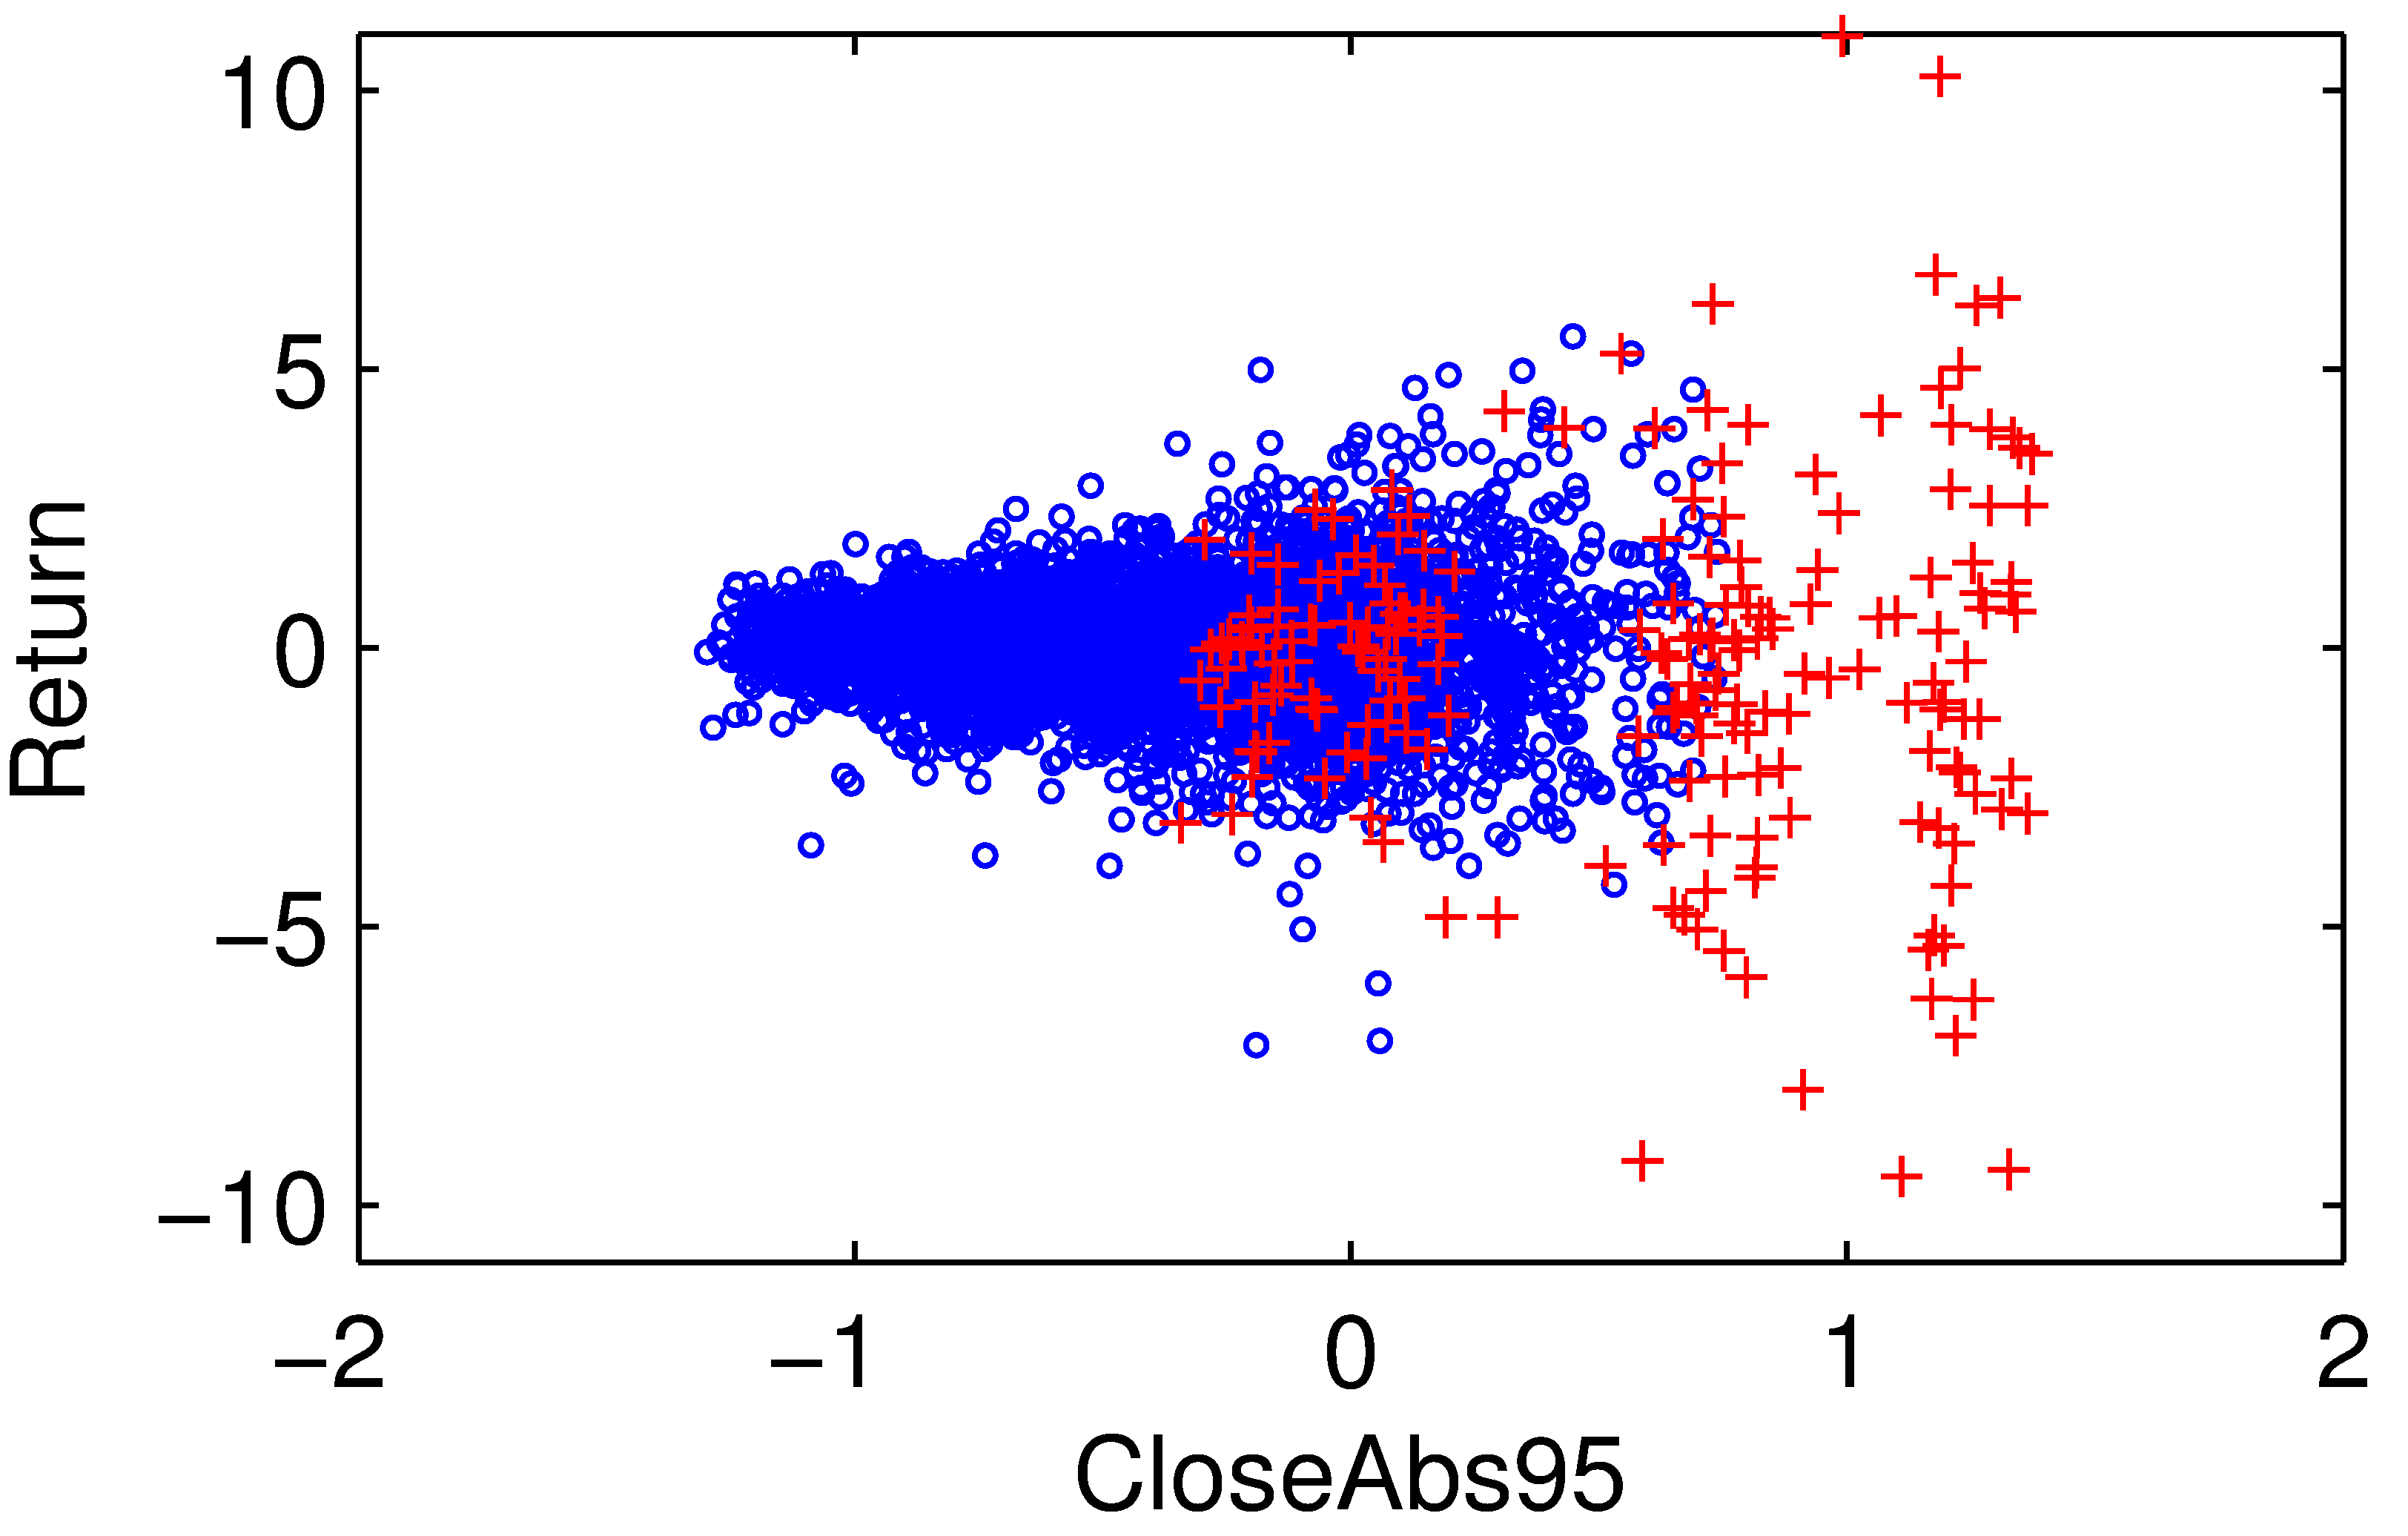
\includegraphics[height=0.8\textheight]{returncloseabs}
  \end{figure}
\end{frame}


\begin{frame}
  \frametitle{The typical data in finance}
  \framesubtitle{Daily stock market returns, a closer look}
  \begin{figure}
    \centering
    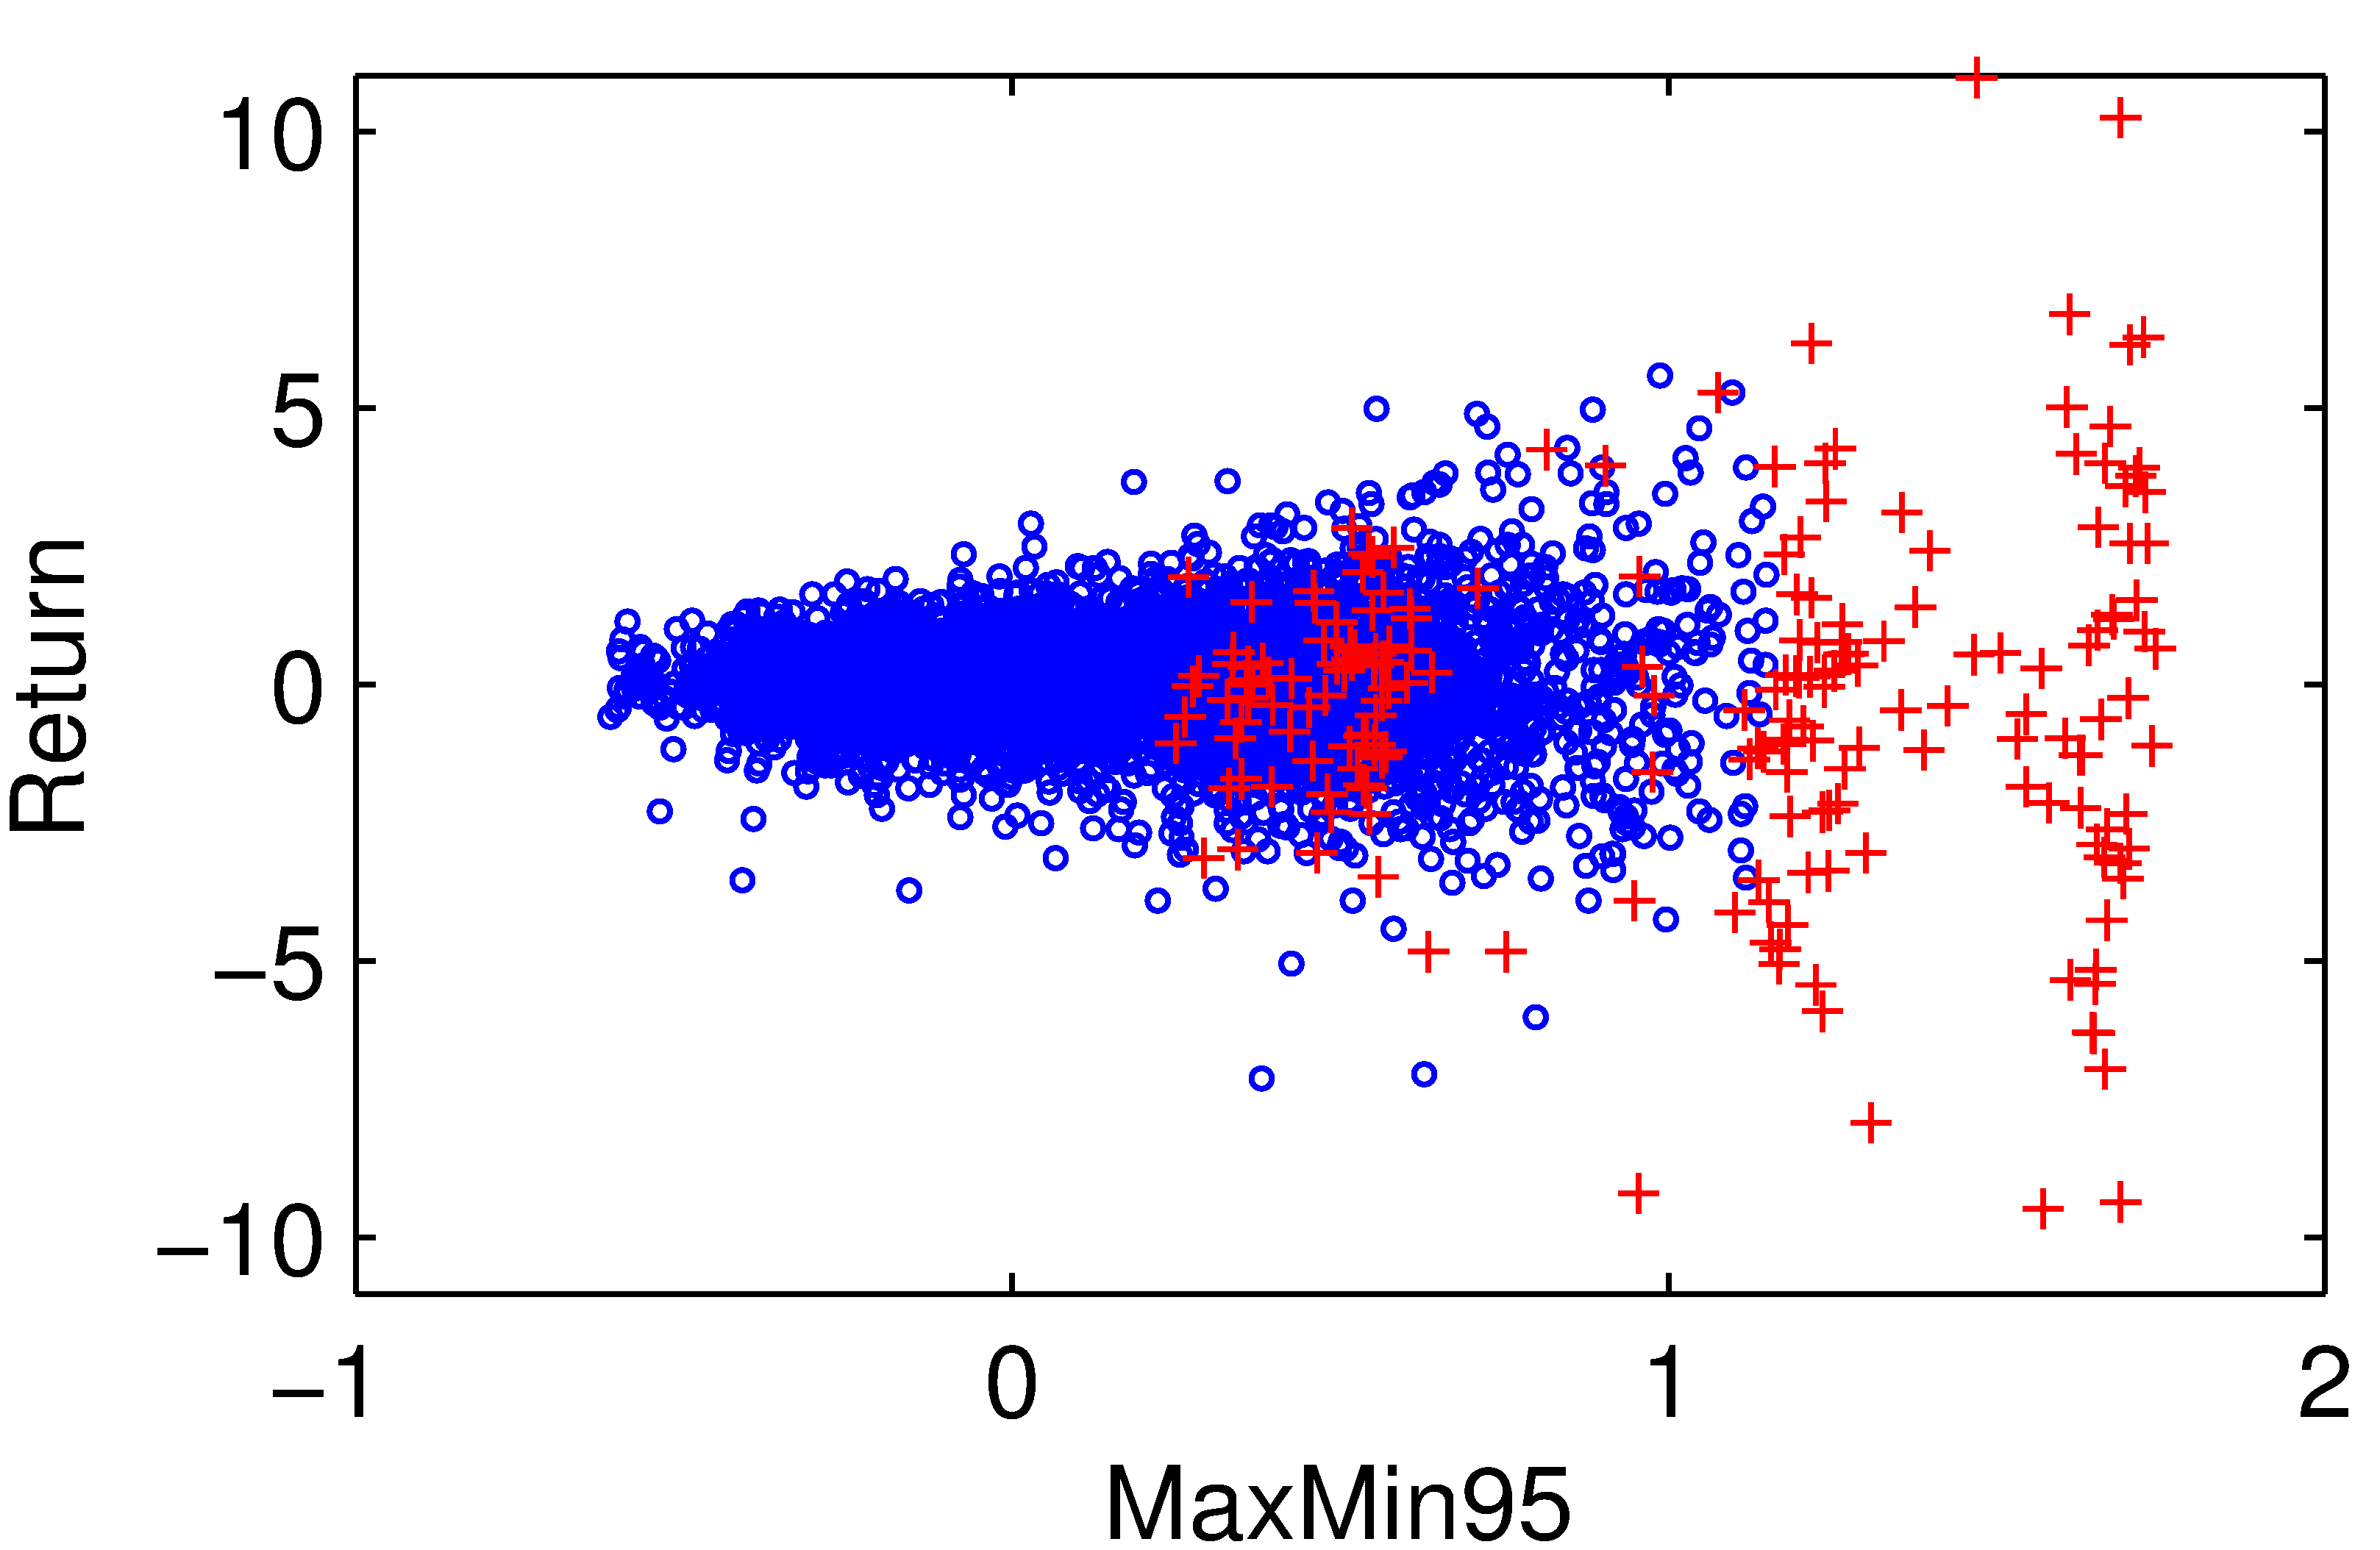
\includegraphics[height=0.8\textheight]{returnminmax}
  \end{figure}
\end{frame}


\begin{frame}
  \frametitle{What can we find?}
  \begin{itemize}
  \item This does not look like as \textbf{normal} (think about the mean and variation)!
  \item How do we describe it in the language of statistics?

    \begin{itemize}
    \item We use \textbf{mean} and \textbf{variance} (\emph{standard deviation}) to describe normality.
    \item We use \textbf{skewness}, and \textbf{kurtosis} (\emph{degrees of freedom}) to detect the
      abnormal events.
    \end{itemize}

  \end{itemize}
\end{frame}

\begin{frame}
  \frametitle{Normal and not normal}
  \begin{figure}
    \centering
    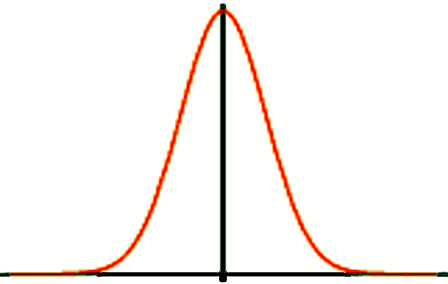
\includegraphics[height=0.42\textheight]{normal}\\
    Normal\\
    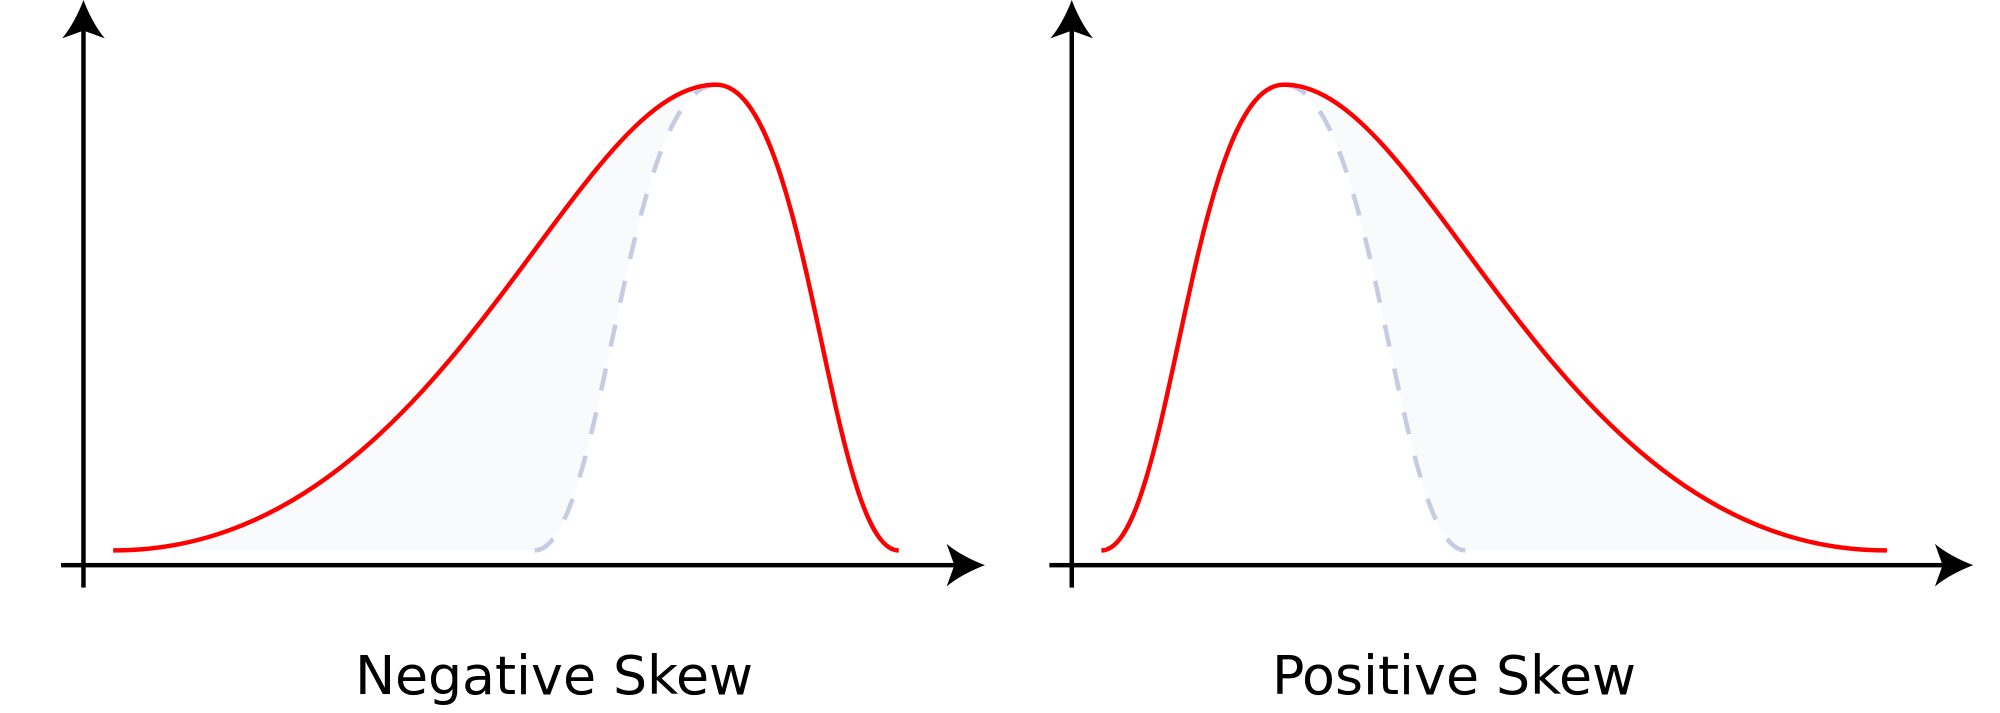
\includegraphics[height=0.42\textheight]{skew}
  \end{figure}
\end{frame}


\begin{frame}
  \frametitle{Detecting the financial crisis}
  \begin{figure}
    \centering
    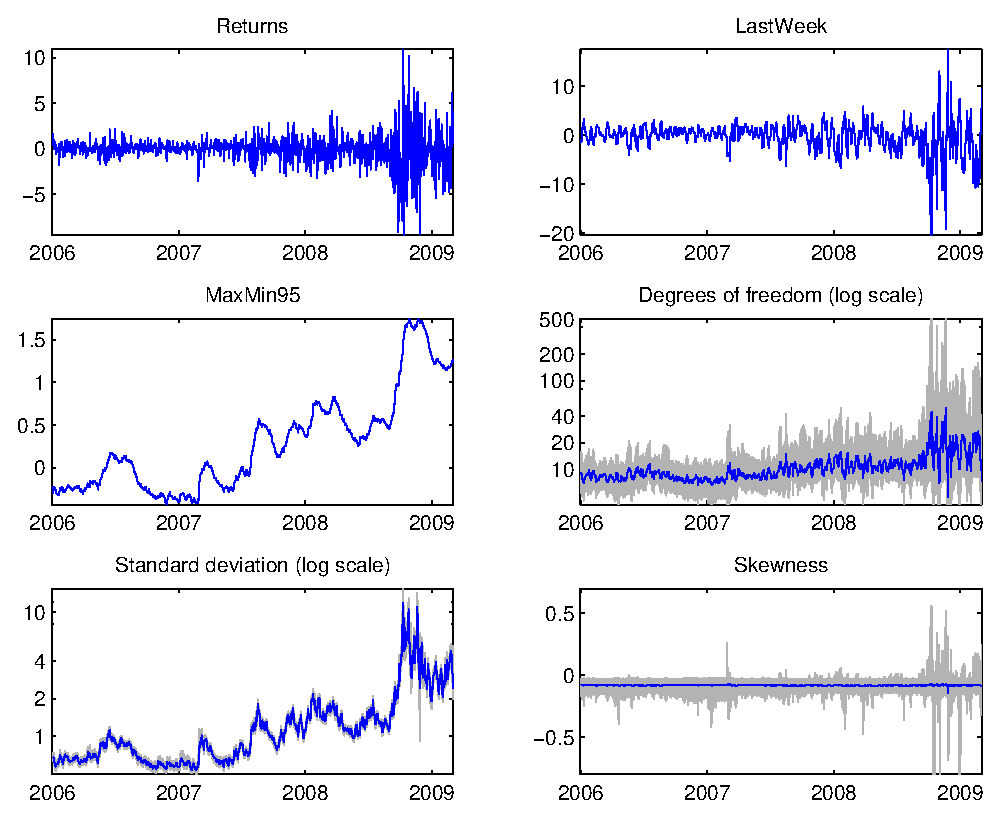
\includegraphics[height=0.9\textheight]{MomentPlotSP5002}
  \end{figure}
\end{frame}


\begin{frame}
  \frametitle{What if we insist using the normal model?}
  \begin{itemize}
  \item The model will be misspecified.
  \item The conclusion based on that model can lead to a wrong decision.
  \item But people still do it anyway!
    \begin{itemize}
    \item The normal model is simpler anyway.
    \item We eventually do not know that we are wrong.
    \item The computational tools are still feasible for everyone to use.
      \begin{itemize}
      \item There was no ready-to-use computer software to use for this model.
      \item The model takes a night to estimate with a cluster.
      \end{itemize}
    \end{itemize}
  \end{itemize}

\end{frame}


\begin{frame}
  \frametitle{A more complicated situation}
  \begin{figure}
    \centering
    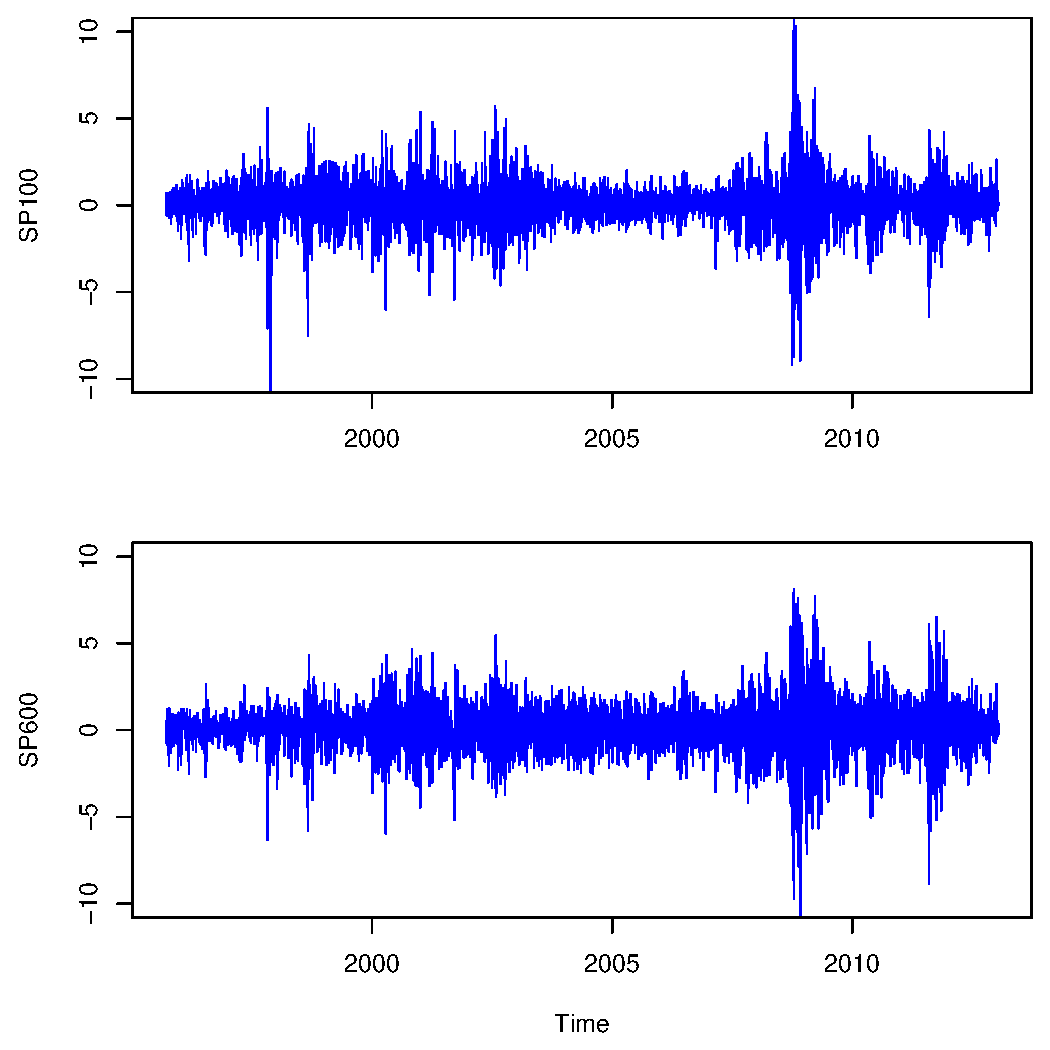
\includegraphics[height=0.9\textheight]{SP100-SP600}
  \end{figure}
\end{frame}

\begin{frame}
  \frametitle{Our interests}

  \begin{itemize}
  \item The S\&P100 index includes the largest and most established companies
    in the U.S.

  \item The S\&P600 index covers the small capitalization companies
which present the possibility of greater capital appreciation, but at greater risk


  \item We are not only interested to detect the extreme events of a single
    stock, but also the co-movement of a two or more stocks.

    \begin{itemize}
    \item What will happen to S\&P100 if S\&P600 collapses?
    \item We call this as \textbf{tail-dependence}---the dependence only
      happens when extreme events happen.
    \item What are the underlying factors that are connected to this dependence?
    \end{itemize}
  \end{itemize}

\end{frame}

\begin{frame}
  \frametitle{The dependence on the tail}
      \begin{figure}
        \centering
        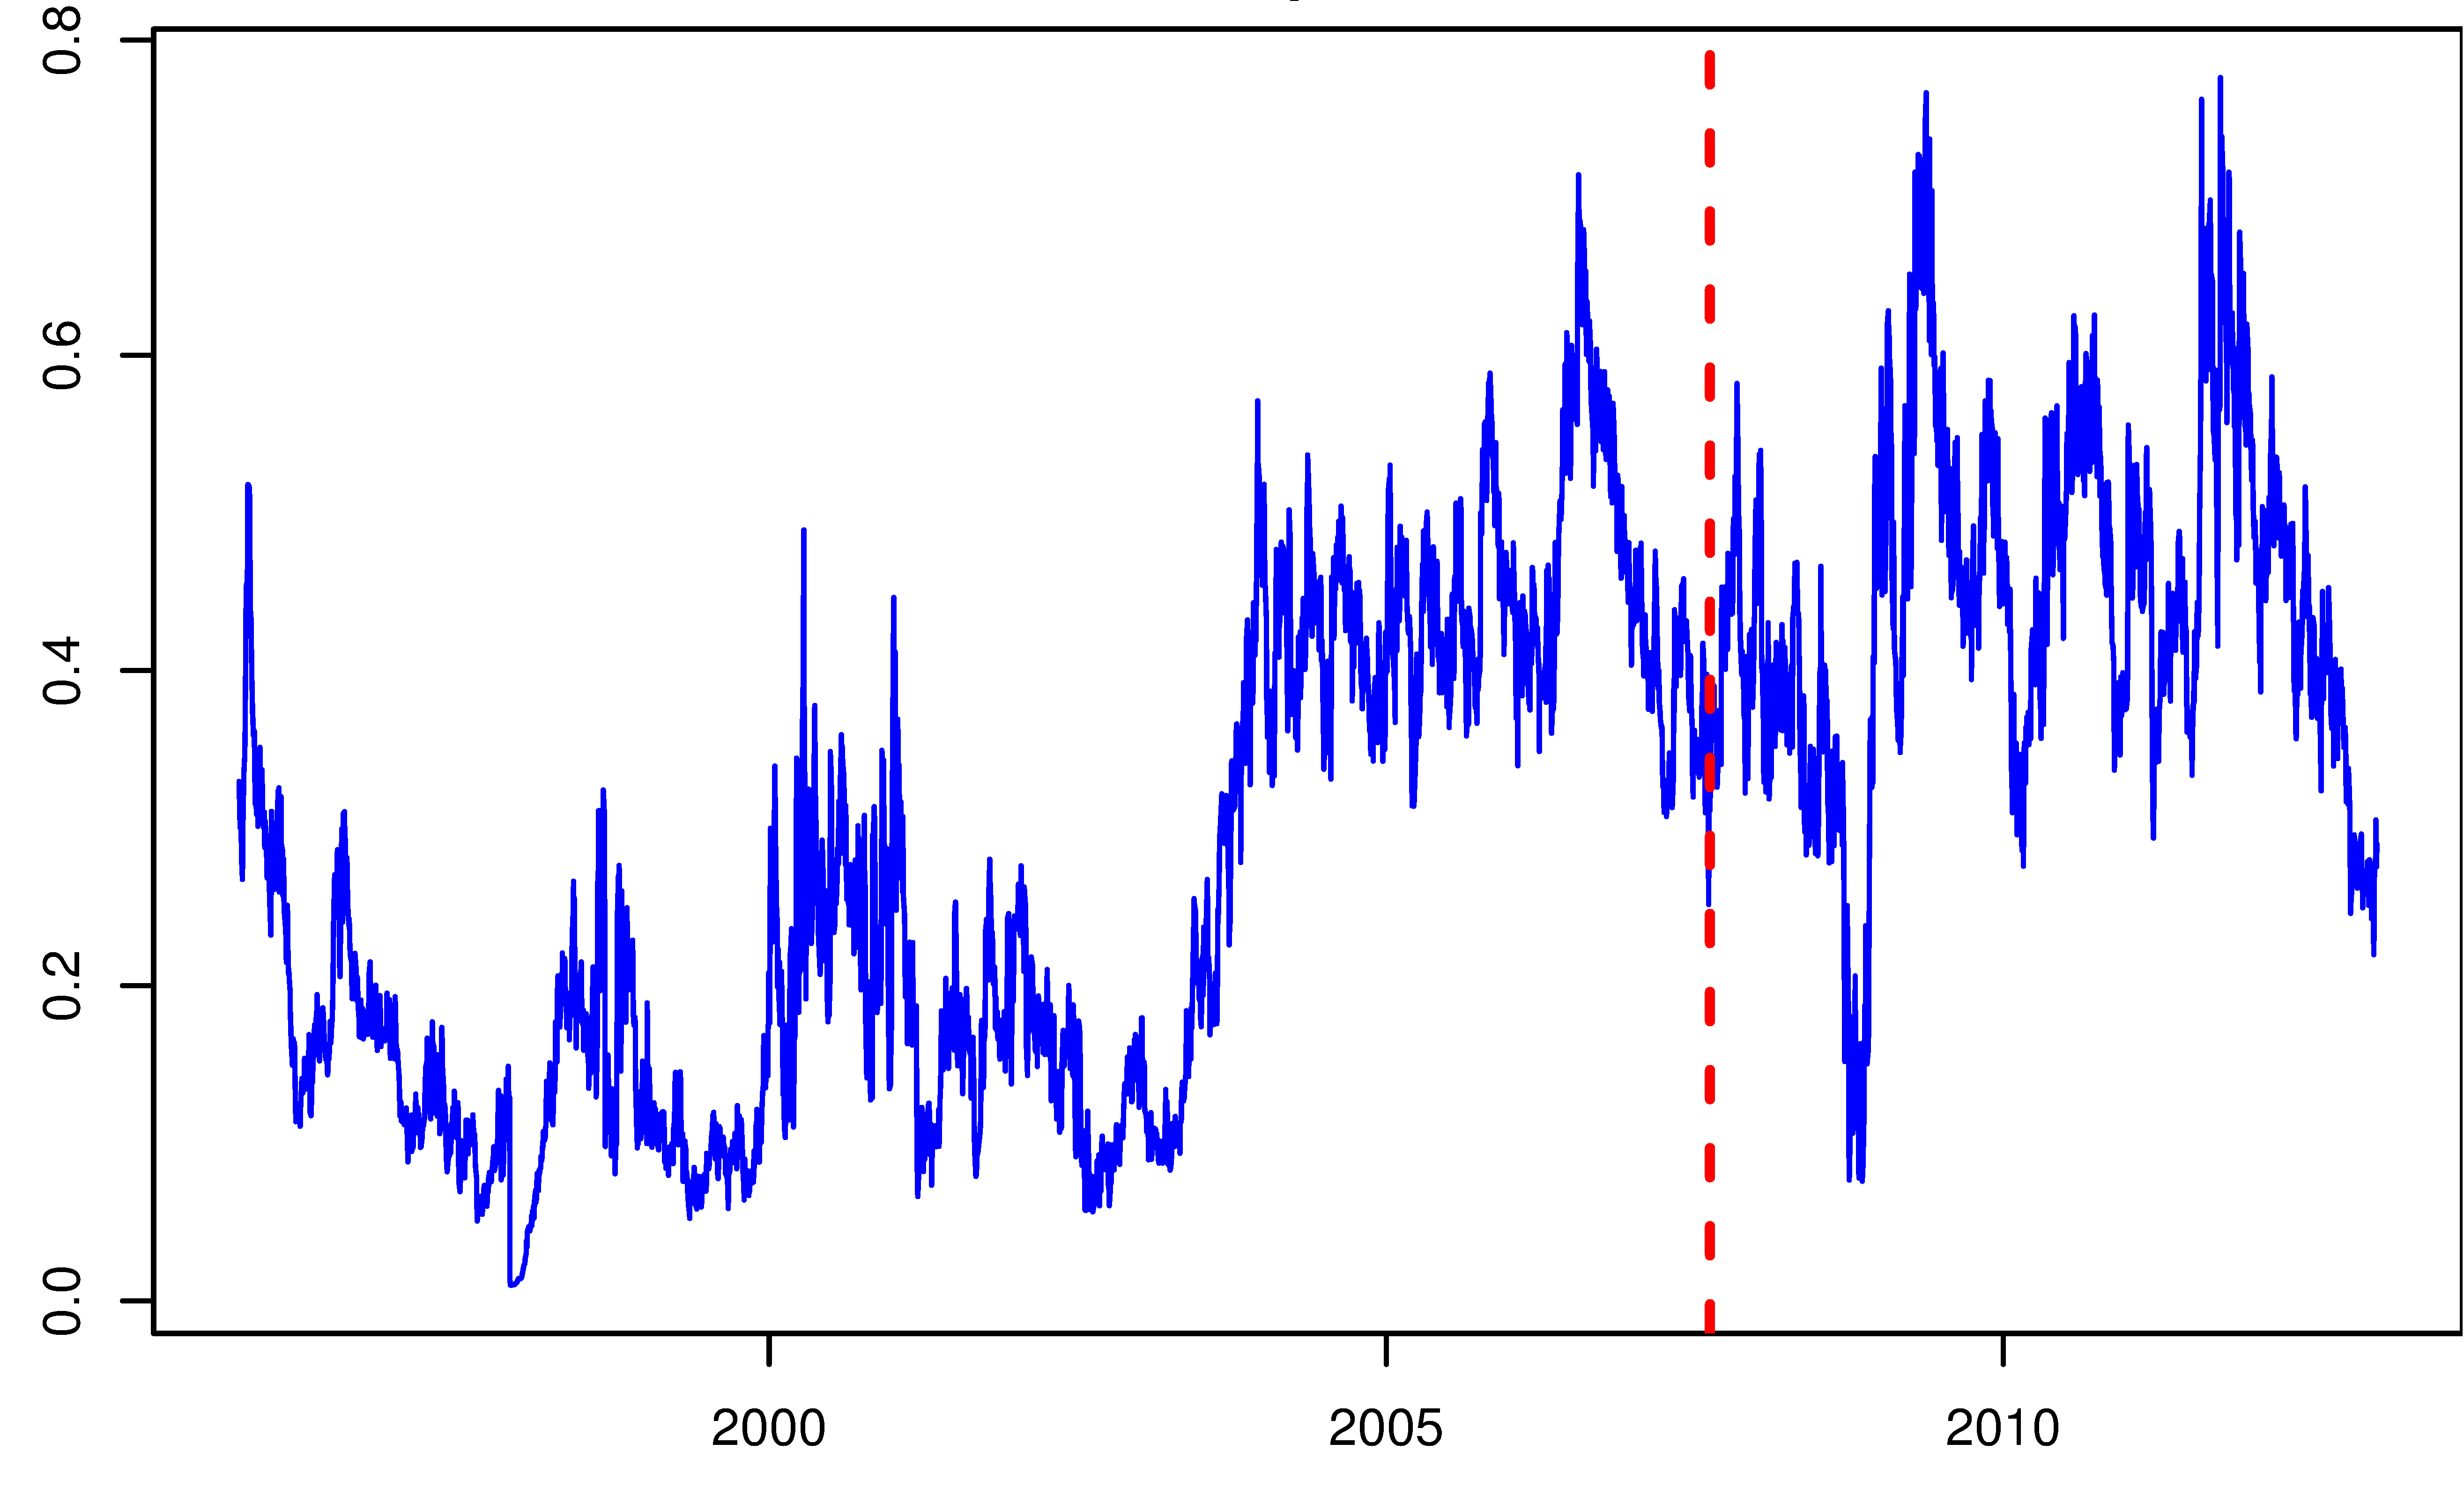
\includegraphics[height=0.8\textheight]{tail-dep}
      \end{figure}
\end{frame}

\begin{frame}
  \frametitle{Knowing the elephant}
  \framesubtitle{The trend of statistical modeling}

  \begin{itemize}
  \item In the 1950s, linear regression model  was considered as very advanced
    which is now the standard course content for university students.
  \item The data are much more complicated nowadays we meet.
    \begin{itemize}
    \item Numerical, categorical, brain image...
    \item A few observations to millions by millions.
    \item Very high-dimensional data are not rare anymore.
    \end{itemize}
  \end{itemize}
\end{frame}



\begin{frame}
  \frametitle{Knowing the elephant}
  \framesubtitle{The common procedure statistical modeling}

  \begin{itemize}
  \item Data collection
  \item Model estimation
  \item Model evaluation
  \item Model comparison
  \item Prediction (if needed)
  \end{itemize}
\end{frame}


\begin{frame}
  \frametitle{Knowing the elephant}
  \framesubtitle{Can we have a model that is big like an elephant?}

      \begin{figure}
        \centering
        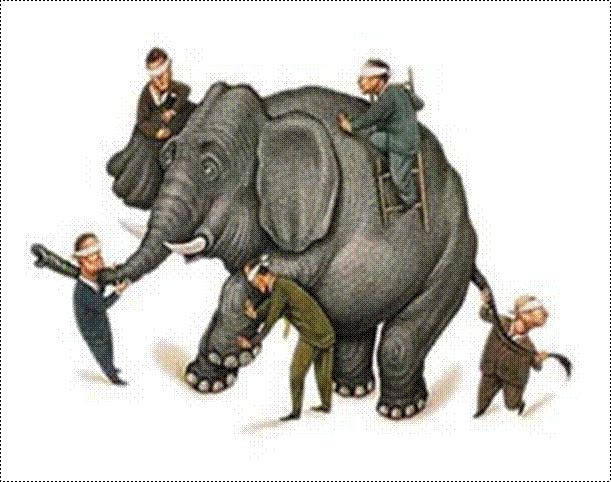
\includegraphics[height=0.8\textheight]{elephant}
      \end{figure}
\tiny{by John Godfrey Saxe (1816-1887)}
\end{frame}


\begin{frame}
  \frametitle{Knowing the elephant}

  \begin{itemize}
  \item Sophisticated models are essential for such situations.
  \item In principle, the complicated model should be able to capture more
    complicated data features.
  \item Estimating such model is not easy.
  \item There is huge space to explore.
    \begin{itemize}
    \item The computer is still not fast enough.
    \item Techniques like parallel
      computing should be used to speed up the computation.
    \item Statistics with big data is the new challenge.
    \end{itemize}
  \end{itemize}
\end{frame}




\begin{frame}[plain]

  \addtocounter{framenumber}{-1}

\emph{...essentially, all models are wrong, but some are useful}\\
\hfill --- George E. P. Box
\vspace{1cm}
  \begin{center}
    {\color{SUblue} \textbf{\Huge Thank you!}}
  \end{center}


\end{frame}




\end{document}
